\section{髮廊服務優化問題 (barbershop)}

\subsection{問題描述}

瑪莉是美美髮廊裡手藝高超的髮型設計師,這天美美髮廊同時來了
\begin{math}n\end{math} 位客人指定瑪莉設計髮型,
因每位客人所指定的服務不同,所需的時間也不盡相同。
一位客人所需等待的時間為他前面所有客人的服務時間與自己服務時間的總和。
為了提高髮廊的服務品質,瑪莉希望這 \begin{math}n\end{math}
位客人總共等待的時間最短, 請幫瑪莉決定服務順序並計算這
\begin{math}n\end{math} 位客人最短的等待時間總和。

假設有三位客人
\begin{math}A\end{math}、\begin{math}B\end{math}、\begin{math}C\end{math},這三位客人分別需要的服務時間為
\begin{math}1\end{math}、\begin{math}2\end{math}、\begin{math}3\end{math}。
如果瑪莉提供服務的順序為 \begin{math}A \to B \to C\end{math},那麼
\begin{math}A\end{math} 需要等待 \begin{math}1\end{math} 分鐘,
\begin{math}B\end{math} 需要等待 \begin{math}1+2 = 3\end{math}
分鐘,\begin{math}C\end{math} 則需要等待 \begin{math}1+2+3=6\end{math}
分鐘。 這三個客人總共等待時間為
\begin{math}1 + (1+2) + (1+2+3) = 10\end{math}。
如果瑪莉提供服務的順序為
\begin{math}C \to B \to A\end{math},那麼這三個客人總共等待時間為
\begin{math}3 + (3+2) + (3+2+1) = 14\end{math}。 因為
\begin{math}10\end{math}
是所有服務順序中總等待時間最短的,因此本例的答案需輸出
\begin{math}10\end{math}。

\subsection{輸入格式}

\begin{format}
\f{
$n$
$t_1$ $t_2$ $\cdots$ $t_n$
}
\end{format}

\begin{itemize}
\tightlist
\item
  \begin{math}n\end{math} 代表客人數量
\item
  \begin{math}t_i\end{math} 為第 \begin{math}i\end{math}
  位客人所需的服務時間
\end{itemize}

\subsection{輸出格式}

\begin{format}
\f{
$S$
}
\end{format}

\begin{itemize}
\tightlist
\item
  \begin{math}S\end{math} 為整數,代表最小的等待時間總和
\end{itemize}

\subsection{測資限制}

\begin{itemize}
\tightlist
\item
  \begin{math}1 \le n \le 200\end{math}
\item
  \begin{math}1 \le t_i \le 200\end{math}
\item
  上述變數皆為整數
\end{itemize}

\subsection{範例測試}

\begin{example}
\exmp{
3
3 1 2
}{%
10
}%
\exmp{
5
5 2 1 4 3
}{%
35
}%
\exmp{
10
9 5 3 4 10 1 7 6 8 2
}{%
220
}%
\end{example}

\subsection{評分說明}

本題共有三組子任務,條件限制如下所示。
每一組可有一或多筆測試資料,該組所有測試資料皆需答對才會獲得該組分數。

\begin{longtable}[]{@{}ccl@{}}
\toprule
子任務 & 分數 & 額外輸入限制 \\
\midrule
\endhead
1 & \(20\) & \begin{math}t_i \le 3\end{math} \\
2 & \(30\) & \begin{math}t_i \le 100\end{math} \\
3 & \(50\) & 無額外限制 \\
\bottomrule
\end{longtable}

\section{校園公車 (bus)}

\subsection{問題描述}

H 大學設有校園公車在固定路線上來回行駛。
想搭乘校園公車的師生或訪客,可以在公車路線上的任意地點以招手方式請駕駛停靠後上車。
由於校園廣大,為方便師生與訪客利用校園公車,校方打算開發一個手機 app,
其中一個服務是透過 GPS
來定位出使用者在校園中的位置,提供最接近的上車地點。

H 大學校園內的任一位置皆能用二維座標 \begin{math}(x, y)\end{math} 表示。
校園公車的路線是由 \begin{math}n\end{math} 條線段所組成,我們以出發點
\begin{math}P_0(x_0, y_0)\end{math}、轉折點
\begin{math}P_1(x_1, y_1), P_2(x_2, y_2), \ldots, P_{n-1}(x_{n-1}, y_{n-1})\end{math}、以及終點
\begin{math}P_n(x_n, y_n)\end{math} 來描述。
在任意兩個相鄰的轉折點之間,公車以直線運行。 以下圖為例,公車路線為
\begin{math}P_0(1, 3), P_1(3, 3), P_2(5, 1), P_3(7, 2), P_4(7, 4), P_5(9, 3)\end{math}。
如果手機使用者在 \begin{math}O_1(2, 1)\end{math},那麼 app
會回報最接近的上車地點在 \begin{math}A(2, 3)\end{math},距離是
\begin{math}2\end{math}; 如果手機使用者在
\begin{math}O_2(5, 0)\end{math},那麼 app 會回報最接近的上車地點在
\begin{math}B(5, 1)\end{math},距離是 \begin{math}1\end{math}。

\begin{figure}[h]
   \centering
   \begin{tikzpicture}[scale=1]
      \filldraw[black] (1, 3) circle (1pt) node[anchor=south east]{\small $P_0$};
      \filldraw[black] (3, 3) circle (1pt) node[anchor=south west]{\small $P_1$};
      \filldraw[black] (5, 1) circle (1pt) node[anchor=east]{\small $P_2$};
      \filldraw[black] (7, 2) circle (1pt) node[anchor=north west]{\small $P_3$};
      \filldraw[black] (7, 4) circle (1pt) node[anchor=south east]{\small $P_4$};
      \filldraw[black] (9, 3) circle (1pt) node[anchor=north west]{\small $P_5$};

      \filldraw[black] (2, 3) circle (1pt) node[anchor=south]{\small $A$};
      \filldraw[black] (5, 1) circle (1pt) node[anchor=south]{\small $B$};
      \draw (1, 3) -- (3, 3);
      \draw (3, 3) -- (5, 1);
      \draw (5, 1) -- (7, 2);
      \draw (7, 2) -- (7, 4);
      \draw (7, 4) -- (9, 3);
      \filldraw[red] (2, 1) circle (1pt) node[anchor=north]{\small $O_1$};
      \filldraw[red] (5, 0) circle (1pt) node[anchor=north]{\small $O_2$};
      \draw[dashed, color=red] (2, 1) -- (2, 3) node[midway,right] {\scriptsize $d=2$};
      \draw[dashed, color=red] (5, 0) -- (5, 1) node[midway,right] {\scriptsize $d=1$};
   \end{tikzpicture}
\end{figure}

給定一位 app
使用者的位置以及校園公車的路線,請寫一支程式來計算該使用者與最近上車地點的距離。

\subsection{輸入格式}

\begin{format}
\f{
$x$ $y$ $n$
$x_0$ $y_0$
$x_1$ $y_1$
\vdots
$x_n$ $y_n$
}
\end{format}

\begin{itemize}
\tightlist
\item
  \begin{math}(x, y)\end{math} 為使用者的位置
\item
  \begin{math}n\end{math} 為校園公車路線的線段數
\item
  \begin{math}(x_0, y_0), (x_1, y_1), \ldots, (x_n, y_n)\end{math}
  為校園公車的路線(包含起點、轉折點與終點)
\end{itemize}

\subsection{輸出格式}

\begin{format}
\f{
$\textrm{ans}$
}
\end{format}

\begin{itemize}
\tightlist
\item
  \begin{math}\textrm{ans}\end{math}
  為一非負浮點數,代表使用者與最近上車地點的距離
\end{itemize}

\subsection{測資限制}

\begin{itemize}
\tightlist
\item
  \begin{math}1 \le n \le 100\end{math}
\item
  \begin{math}0\le x, y\le10^6\end{math}
\item
  對於所有的 \begin{math}i\in\{0, 1, \ldots, n\}\end{math},皆有
  \begin{math}0 \le x_i, y_i \le 10^6\end{math}
\item
  對於所有的 \begin{math}i\in\{0, 1, \ldots, n-1\}\end{math},皆有
  \begin{math}(x_i, y_i)\ne(x_{i+1}, y_{i+1})\end{math}
\item
  輸入的數皆為整數
\end{itemize}

\subsection{範例測試}

\begin{example}
\exmp{
2 1 5
1 3
3 3
5 1
7 2
7 4
9 3
}{%
2
}%
\exmp{
5 0 5
1 3
3 3
5 1
7 2
7 4
9 3
}{%
1
}%
\exmp{
10 3 1
4 4
9 4
}{%
1.414213562373095
}%
\exmp{
10 3 2
9 4
9 13
10 13
}{%
1.414213562373095
}%
\end{example}

\subsection{評分說明}

本題共有三組子任務,條件限制如下所示。
每一組可有一或多筆測試資料,該組所有測試資料皆需答對才會獲得該組分數。
若正確答案非 \begin{math}0\end{math},輸出和正確答案的絕對或相對誤差在
\begin{math}10^{-6}\end{math} 就算正確。 若答案為
\begin{math}0\end{math},輸出必須要和正確答案絕對誤差在
\begin{math}10^{-6}\end{math} 以內。

\begin{longtable}[]{@{}ccl@{}}
\toprule
子任務 & 分數 & 額外輸入限制 \\
\midrule
\endhead
1 & \(30\) & 校園公車路線為一垂直或水平線段,且所有座標皆在
\begin{math}100\end{math} 以內 \\
2 & \(30\) & 校園公車路線的每一個線段都是垂直或水平 \\
3 & \(40\) & 無額外條件限制 \\
\bottomrule
\end{longtable}

\section{街頭藝人 (busker)}

\subsection{問題描述}

阿甘是一位街頭藝人,他到各地旅行,沿途表演賺取生活花費。

此次阿甘旅行到妙世界國,妙世界國的地圖上有很多節點,每個節點可以細分成兩種:都市和村莊。
已知妙世界國有 \begin{math}n\end{math} 座都市,都市的節點編號分別為
\(1, 2, \cdots, n\), 有 \begin{math}m\end{math}
條\textbf{單向}大道連接這些都市,
每條大道單向連接兩相異都市,並且在都市間會經過\textbf{恰} \(k\) 座村莊。
第 \begin{math}j\end{math} 條大道沿途經過的村莊節點編號分別為
\((n + (j-1)k + 1), (n + (j-1)k + 2), \cdots, (n + jk)\)。

阿甘正思索著要如何規劃一條演藝路線。
演藝路線必須從一個節點開始,沿著大道經過其他節點,
且沿途去過的節點不再經過,最後再回到一開始出發的節點。

另外,各地的物價有所不同,有時表演得到的小費足以應付他的開支,有時卻不夠,
已知編號 \begin{math}i\end{math} 的節點表演所獲取的總收支為
\begin{math}c_i\end{math} 元,
阿甘希望在這條演藝路線上,不能有入不敷出的情況發生,
也就是說如果一條演藝路線經過的節點依序是
\begin{math}\delta_1, \delta_2, \cdots, \delta_r\end{math} (其中
\begin{math}\delta_1=\delta_r\end{math}), 那對所有整數
\begin{math}y \in [1, r]\end{math} 要滿足
\begin{math}\sum_{x=1}^y c_{\delta_x} \geq 0\end{math}。
阿甘把這種演藝路線叫做\textbf{入能敷出演藝路線}。

下圖的例子中有
\begin{math}m = 6\end{math}、\begin{math}n = 5\end{math}、\begin{math}k = 1\end{math}。圖中的紅色圓圈代表都市節點,藍色方形代表村莊節點。圓圈與方形中的數字代表進入此節點後會得到的收支。節點右上角的數字則代表節點編號。

\begin{figure}[h]
  \centering
  \begin{tikzpicture}[scale=1.5,square/.style={regular polygon,regular polygon sides=4}]
    \def \Nodes {
      1/2/2/5,
      2/4/0/-1,
      3/6/2/3,
      4/4/4/2,
      5/0/4/-5,
      6/3/1/0,
      7/5/1/-4,
      10/3/3/-3,
      8/5/3/-3,
      9/4/2/-1,
      11/1/3/3}
    \def \Edges {
      6/1,
      1/10,
      11/1,
      2/6,
      7/2,
      9/2,
      3/7,
      8/3,
      4/8,
      4/9,
      10/4,
      5/11}

    \foreach \id / \x / \y / \w in \Nodes {
      \def \shape{\directlua{
        if \id <= 5 then
          tex.sprint("circle")
        else
          tex.sprint("square")
        end
      }}
      \def \color{\directlua{
        if \id <= 5 then
          tex.sprint("red!50")
        else
          tex.sprint("blue!50")
        end
      }}
      \def \xb{\directlua{
        tex.sprint(\x + 0.5)
      }}
      \def \yb{\directlua{
        tex.sprint(\y + 0.5)
      }}
      \node[draw,\shape,fill=\color,minimum size=1cm] (\id) at (\x, \y) {\small \w};
      \node[text width=1cm] at (\xb, \yb) {\small \id};
    }
    \foreach \x / \y in \Edges {
      \path[draw,->,thick] (\x) -- (\y);
    }
  \end{tikzpicture}
  \caption{圖一}
\end{figure}

一條入能敷出演藝路線可以依序經過都市 \begin{math}1\end{math}
(此時阿甘口袋有 \begin{math}5\end{math} 元)、 村莊
\begin{math}10\end{math} (口袋剩 \begin{math}5-3 = 2\end{math} 元)、都市
\begin{math}4\end{math} (口袋剩 \begin{math}2+2 = 4\end{math} 元)、 村莊
\begin{math}9\end{math} (口袋剩 \begin{math}4-1 = 3\end{math} 元)、都市
\begin{math}2\end{math} (口袋剩 \begin{math}3-1 = 2\end{math} 元)、 村莊
\begin{math}6\end{math} (口袋剩 \begin{math}2+0 = 2\end{math}
元),而最後回到都市 \begin{math}1\end{math} (口袋剩
\begin{math}2+5 = 7\end{math} 元),沿途都沒有入不敷出的狀況。

如果兩條演藝路線經過的的大道集合相同只是起點不同,我們說這兩條演藝路線\textbf{在同一個迴路上}。

若和前一個例子在同一個迴路上,從都市 \begin{math}4\end{math}
出發或是村莊 \begin{math}6\end{math} 出發,也是入能敷出演藝路線。
但從村莊 \begin{math}9\end{math}
出發第一站便入不敷出,不是入能敷出演藝路線。

由於妙世界國很龐大,手算過於耗時,阿甘拜託你幫忙輸出任何一條入能敷出演藝路線,
並計算在同一個迴路上有幾個都市和幾個村莊可以當作入能敷出演藝路線的起始節點。

\subsection{輸入格式}

\begin{format}
\f{
$n$ $m$ $k$
$c_1$
$c_2$
$\vdots$
$c_n$
$x_1$ $y_1$ $c_{n+1}$ $c_{n+2}$ $\cdots$ $c_{n+k}$
$x_2$ $y_2$ $c_{n+k+1}$ $c_{n+k+2}$ $\cdots$ $c_{n+2k}$
$\vdots$
$x_{m}$ $y_{m}$ $c_{n+(m-1)k+1}$ $c_{n+(m-1)k+2}$ $\cdots$ $c_{n+mk}$
}
\end{format}

\begin{itemize}
\tightlist
\item
  \begin{math}n\end{math} 代表都市數量。
\item
  \begin{math}m\end{math} 代表單向大道數量。
\item
  \begin{math}k\end{math} 代表每條單向大道上有幾個村莊。
\item
  \begin{math}c_i\end{math} 代表在第 \begin{math}i\end{math}
  個節點表演的收支。
\item
  \begin{math}x_j\end{math} 代表第 \begin{math}j\end{math}
  條單向大道的起點都市。
\item
  \begin{math}y_j\end{math} 代表第 \begin{math}j\end{math}
  條單向大道的終點都市。
\end{itemize}

\subsection{輸出格式}

請依照以下格式輸出一組入能敷出演藝路線。若存在多組入能敷出演藝路線,輸出任意一組即可:

\begin{format}
\f{
$r$
$\delta_1$ $\delta_2$ $\cdots$ $\delta_r$
$city$ $village$
}
\end{format}

\begin{itemize}
\tightlist
\item
  \begin{math}r\end{math} 代表入能敷出演藝路線走過的節點數量
\item
  \begin{math}\delta_i\end{math} 代表入能敷出演藝路線的第
  \begin{math}i\end{math} 站的節點編號
\item
  輸出必須滿足 \begin{math}\delta_1 = \delta_r\end{math}
\item
  \begin{math}city\end{math}
  代表在同一個迴路上有幾個都市可以當入能敷出演藝路線的起始節點
\item
  \begin{math}village\end{math}
  代表在同一個迴路上有幾個村莊可以當入能敷出演藝路線的起始節點
\item
  輸出的數皆為整數
\end{itemize}

若不存在入能敷出演藝路線,則輸出唯一一行 \begin{math}0\end{math}:

\begin{format}
\f{
$0$
}
\end{format}

\subsection{測資限制}

\begin{itemize}
\tightlist
\item
  \begin{math}1 \le n \le 2000\end{math}
\item
  \begin{math}1 \le m \le 8000\end{math}
\item
  \begin{math}1 \le k \le n\end{math}
\item
  \begin{math}-10^8 \le c_i \le 10^8\end{math}
\item
  對所有整數 \(j \in [1, m]\) 保證 \begin{math}x_j \neq y_j\end{math}
\item
  對所有整數 \(a, b \in [1, m]\) 保證若 \begin{math}a \neq b\end{math}
  則 \begin{math}x_a \neq x_b\end{math} 或
  \begin{math}y_a \neq y_b\end{math}
\item
  輸入的數皆為整數
\end{itemize}

\subsection{範例測試}

\begin{example}
\exmp{
5 6 1
5
-1
3
2
-5
2 1 0
3 2 -4
4 3 -3
4 2 -1
1 4 -3
5 1 3
}{%
7
6 1 10 4 9 2 6
2 1
}%
\exmp{
2 2 1
-1
-1
1 2 1
2 1 0
}{%
0
}%
\exmp{
2 2 1
-1
-1
1 2 1
2 1 1
}{%
5
4 1 3 2 4
0 2
}%
\end{example}

\subsection{評分說明}

本題共有三組子任務,條件限制如下所示。
每一組可有一或多筆測試資料,該組所有測試資料皆需答對才會獲得該組分數。

\begin{longtable}[]{@{}ccl@{}}
\toprule
子任務 & 分數 & 額外輸入限制 \\
\midrule
\endhead
1 & \(18\) & \begin{math}n \le 20\end{math} \\
2 & \(15\) & \begin{math}n \le 90\end{math} \\
3 & \(67\) & 無額外限制 \\
\bottomrule
\end{longtable}

\section{汽車不再繞圈圈 (car)}

\subsection{問題描述}

小戸川市以觀光和計程車的發達聞名,外國遊客們常常在城巿裡搭計程車往返各個景點。
城巿裡的道路交通網是一個有向圖(directed
graph),每條道路的通行方向可以透過特殊的權限由主控台改變。
詳細一點來說,城市共有 \begin{math}n\end{math} 個景點(編號由
\begin{math}1\end{math} 至 \begin{math}n\end{math})與
\begin{math}m\end{math} 條道路(編號由 \begin{math}1\end{math} 到
\begin{math}m\end{math})。 第 \begin{math}i\end{math} 條道路由
\begin{math}u_i\end{math} 單向通往
\begin{math}v_i\end{math},並且需要至少 \begin{math}c_i\end{math}
(\begin{math}c_i \ge 1\end{math})的管理者權限才能改變方向。
管理權限可以由一個正整數表示,數字越大代表權限越大; 若管理者有
\begin{math}P\end{math} 的權限,則他可以透過系統改變任意
\begin{math}c_i \le P\end{math} 的道路方向。

某天小戸川市的交通局被觀光客投訴部份計程車司機會利用城巿裡的道路載著乘客繞圈圈以收取更高的費用。
為了避免這個亂象,城巿的交通局長決定透過改變城市中某些道路的方向,使得城市中不存在環,讓計程車司機們無法在城巿裡繞圈圈。
交通局長請資訊專長的你幫忙計算至少要多大的權限才能達成目標。
請注意由於城市的都市規劃不佳,兩景點間可能有複數條道路存在或者完全無法到達的情況發生。

以下圖為例,其中邊上的數字代表改變該條道路方向所需的權限,
若管理者權限為 \begin{math}2\end{math},並改變
\begin{math}(2,1)\end{math}、\begin{math}(2,3)\end{math}
這兩條道路的方向即可達成目標。
這也是能達成交通局長目標的管理者權限最小值。

\begin{minipage}{0.49\textwidth}
  \begin{figure}[H]
    \centering
    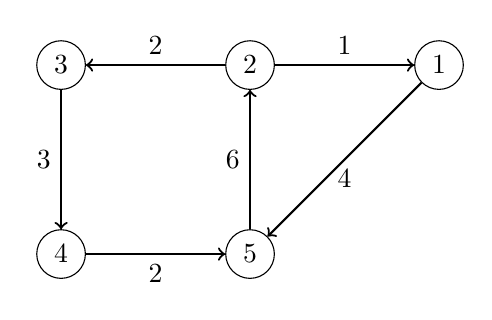
\begin{tikzpicture}[scale=0.8]
      \def \Nodes {
        1/6/3,
        2/3/3,
        3/0/3,
        4/0/0,
        5/3/0}
      \def \Edges {
        2/1/1/above,
        1/5/4/below,
        5/2/6/left,
        2/3/2/above,
        3/4/3/left,
        4/5/2/below}

      \foreach \id / \x / \y in \Nodes {
        \node[draw,circle] (\id) at (\x, \y) {\id};
      }
      \foreach \x / \y / \w / \labelpos in \Edges {
        \path[draw,->,thick] (\x) -- (\y) node[midway,\labelpos] {\w};
      }
    \end{tikzpicture}
    \caption{改變道路方向前}
  \end{figure}
\end{minipage}
\begin{minipage}{0.49\textwidth}
  \begin{figure}[H]
    \centering
    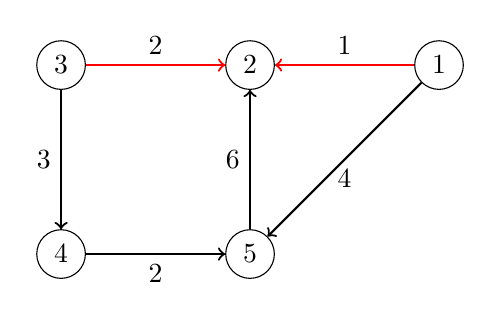
\begin{tikzpicture}[scale=0.8]
      \def \Nodes {
        1/6/3,
        2/3/3,
        3/0/3,
        4/0/0,
        5/3/0}
      \def \Edges {
        1/2/1/above/red,
        1/5/4/below/black,
        5/2/6/left/black,
        3/2/2/above/red,
        3/4/3/left/black,
        4/5/2/below/black}

      \foreach \id / \x / \y in \Nodes {
        \node[draw,circle] (\id) at (\x, \y) {\id};
      }
      \foreach \x / \y / \w / \labelpos / \color in \Edges {
        \path[draw=\color,->,thick] (\x) -- (\y) node[midway,\labelpos] {\w};
      }
    \end{tikzpicture}
    \caption{改變道路方向後}
  \end{figure}
\end{minipage}

\subsection{輸入格式}

\begin{format}
\f{
$n$ $m$
$u_1$ $v_1$ $c_1$
$u_2$ $v_2$ $c_2$
$\vdots$
$u_m$ $v_m$ $c_m$
}
\end{format}

\begin{itemize}
\tightlist
\item
  \begin{math}n\end{math}、\begin{math}m\end{math}
  分別代表城市數與道路數
\item
  \begin{math}u_i\end{math}、\begin{math}v_i\end{math}、\begin{math}c_i\end{math}
  代表第 \begin{math}i\end{math} 條道路單向連接
  \begin{math}u_i\end{math} 到
  \begin{math}v_i\end{math},且改變方向需要的權限為
  \begin{math}c_i\end{math}
\end{itemize}

\subsection{輸出格式}

\begin{format}
\f{
$P$ $R$
$e_1$
$e_2$
$\vdots$
$e_R$
}
\end{format}

\begin{itemize}
\tightlist
\item
  \begin{math}P\end{math}
  為一整數,代表達成交通局長目標需要最少的權限大小。若不需要改變任何道路方向即可達成交通局長的要求,\begin{math}P\end{math}
  請輸出 \begin{math}0\end{math}
\item
  \begin{math}R\end{math} 為一整數,代表需要改變方向的道路個數
\item
  \begin{math}e_i\end{math} 為一整數,代表第 \begin{math}i\end{math}
  條想要改變方向的道路編號。注意同一條道路編號不可以在
  \begin{math}e\end{math}
  出現兩次以上,並且改變此條道路所需的權限也不可以超過
  \begin{math}P\end{math}(意即必須滿足
  \begin{math}c_{e_i} \le P\end{math})
\end{itemize}

請注意雖然輸出的權限大小必須最小,但改變的道路數量可以是任意數量。
若有多組改變方案可以滿足要求,請輸出任意一組即可。

\subsection{測資限制}

\begin{itemize}
\tightlist
\item
  \begin{math}2 \le n \le 10^5\end{math}
\item
  \begin{math}0 \le m \le 10^5\end{math}
\item
  \begin{math}1 \le u_i, v_i \le n\end{math},且
  \begin{math}u_i \neq v_i\end{math}(\begin{math}i \in \{1, 2, \ldots, m\}\end{math})
\item
  \begin{math}1 \le c_i \le 10^9\end{math}(\begin{math}i \in \{1, 2, \ldots, m\}\end{math})
\item
  上面所有變數皆為整數
\end{itemize}

\subsection{範例測試}

\begin{example}
\exmp{
5 6
2 1 1
1 5 4
5 2 6
2 3 2
3 4 3
4 5 2
}{%
2 2
1
4
}%
\exmp{
2 1
1 2 6
}{%
0 0
}%
\exmp{
6 7
5 2 6
2 1 1
2 3 10
3 4 3
4 5 2
1 5 4
4 5 1
}{%
2 3
2
5
7
}%
\end{example}

\subsection{評分說明}

本題共有三組子任務,條件限制如下所示。
每一組可有一或多筆測試資料,該組所有測試資料皆需答對才會獲得該組分數。

\begin{longtable}[]{@{}ccl@{}}
\toprule
子任務 & 分數 & 額外輸入限制 \\
\midrule
\endhead
1 & \(6\) & \begin{math}n,m \le 20\end{math} \\
2 & \(8\) & \begin{math}c_i \le 100\end{math} \\
3 & \(86\) & 無額外限制 \\
\bottomrule
\end{longtable}

\section{天空競技場 (colosseum)}

\subsection{問題描述}

臘月寒冬,小傑來到天空競技場磨練競技程式的技術並賺取金幣。
天空競技場是一棟非常高的建築物,遠遠看去彷彿有一百萬層那麼高。
小傑來到的競技場是一棟 \begin{math}n\end{math} 層樓的建築物,樓層標號為
\begin{math}1\end{math} 到
\begin{math}n\end{math},樓層編號越大代表所在位置越上面。 參加者會在時間
\begin{math}0\end{math}
時選擇任一樓層作為起點進入或直接離開放棄挑戰,並可以在任意時間點任意樓層選擇結束挑戰並獲得累積的金幣獎勵。
進到競技場後,參賽者會從選擇的起點樓層開始一層一層往上直到離開,到結束挑戰前都不可跳過樓層也不可以往下面樓層走。
競技場設有高速移動的電梯,可以讓參賽者一瞬間移動到樓上一層,所以樓層之間的移動時間可以視為
\begin{math}0\end{math} 不計。

競技場每個樓層都有一位樓主,第 \begin{math}i\end{math} 層的開設時間為
\begin{math}x_i\end{math},挑戰門檻為 \begin{math}y_i\end{math}。
參加者到樓層 \begin{math}i\end{math} 時若所持金幣未滿
\begin{math}y_i\end{math}
則無法參加這個樓層的競技,參加者只能繼續往上走或結束挑戰。
任何滿足金幣門檻(所持金幣 \begin{math}y_i\end{math}
以上)的參加者如果恰在開設時間 \begin{math}x_i\end{math} 或之後到達第
\begin{math}i\end{math} 樓的話就會強制發生戰鬥與樓主競技,不能拒絕。
此競技將耗費 \begin{math}t_i\end{math} 的時間並於競技結束時獲取
\begin{math}w_i\end{math} 的金幣。 如果在時間 \begin{math}x_i\end{math}
之前到達 \begin{math}i\end{math}
樓且滿足金幣門檻的參賽者,則可以選擇在這層樓等待至開設時間或是直接繼續往上走。

小傑對競技場的挑戰非常感興趣,但不巧他今天得在時間
\begin{math}m\end{math} 或以前離開競技場回去參加程式比賽,
請幫小傑規劃從哪一個樓層開始以及要在哪些樓層等待,讓他可以在
\begin{math}m\end{math} 的時間內得到最多的金幣。

\newpage

下面是一個 \begin{math}n=6, m=9\end{math} 的例子,
左方表格內是各樓層的開始時間 \begin{math}x_i\end{math}、門檻值
\begin{math}y_i\end{math}、競技耗時 \begin{math}t_i\end{math} 與可獲金幣
\begin{math}w_i\end{math},右圖中列舉了三種可能(但非全部)的路線。 (a)
路線從 \begin{math}1\end{math} 樓進入,因為到達時
\begin{math}1\end{math}
樓已達開設時間且滿足挑戰門檻所以必須競技,在一樓耗費
\begin{math}4\end{math} 時間獲得 \begin{math}1\end{math} 金幣。
然後依序在 \begin{math}2,3\end{math} 樓獲得 \begin{math}3\end{math} 與
\begin{math}1\end{math} 枚金幣。在時間 \begin{math}9\end{math} 時共獲得
\begin{math}5\end{math} 枚金幣離開。 (b) 路線由 \begin{math}2\end{math}
樓進入,先在 \begin{math}2\end{math} 樓等到
\begin{math}x_2 = 1\end{math} 時參加競技,耗費 \begin{math}2\end{math}
時間獲得 \begin{math}3\end{math} 金幣。 到達 \begin{math}3\end{math}
樓時因為門檻不滿足直接進入 \begin{math}4\end{math}
樓,\begin{math}4\end{math} 樓的開始時間 \begin{math}x_4=6\end{math}
未到,選擇不等待直接進入 \begin{math}5\end{math} 樓, 之後等待
\begin{math}1\end{math} 時間與耗費 \begin{math}5\end{math} 時間獲得
\begin{math}5\end{math} 枚金幣,總共獲取 \begin{math}8\end{math}
枚金幣離開,這是本例中可獲得最多金幣的策略之一。

\begin{minipage}{0.35\textwidth}
\begin{table}[H]
  \centering
  \begin{tabular}{|c|c|c|c|c|}
  \hline
  $i$ & $x_i$ & $y_i$ & $t_i$ & $w_i$ \\
  \hline
  $6$ & $1$ & $0$ & $7$ & $6$ \\
  \hline
  $5$ & $4$ & $3$ & $5$ & $5$ \\
  \hline
  $4$ & $6$ & $1$ & $1$ & $4$ \\
  \hline
  $3$ & $2$ & $4$ & $3$ & $1$ \\
  \hline
  $2$ & $1$ & $0$ & $2$ & $3$ \\
  \hline
  $1$ & $0$ & $0$ & $4$ & $1$ \\
  \hline
  \end{tabular}
  \caption{各樓層的開始時間及門檻}
\end{table}
\end{minipage}
\hfill
\begin{minipage}{0.64\textwidth}
  \begin{figure}[H]
  \begin{tikzpicture}[scale=0.9]
    \draw[help lines, color=gray!30, dashed] (0, 0) grid (10, 9);
    \draw[->, ultra thick] (0, 0) -- (10, 0) node[right]{時間};
    \draw[->, ultra thick] (0, 0) -- (0, 9) node[above]{樓層};
    \draw[blue, ultra thick] (9, -0.5) -- (9, 9.5) node[above]{$m=9$};

    \draw[->, thick] (0, 1) -- node[above]{\footnotesize 1F競技 (1\$)} (4, 1);
    \draw[->, thick] (4, 1) -- (4, 2);
    \draw[->, thick] (4, 2) -- node[above]{\footnotesize 2F競技 (3\$)} (6, 2);
    \draw[->, thick] (6, 2) -- (6, 3);
    \draw[->, thick] (6, 3) -- node[above]{\footnotesize 3F競技 (1\$)} (9, 3) node[right] {(a)};

    \draw[->, red, thick] (0, 2) -- node[above]{\footnotesize 等待} (1, 2);
    \draw[->, red, thick] (1, 2) -- node[above]{\footnotesize 2F (3\$)} (3, 2);
    \draw[->, red, thick] (3, 2) -- (3, 3);
    \draw[->, red, thick] (3, 3) -- node[right]{\footnotesize 上5F} (3, 4);
    \draw[->, red, thick] (3, 4) -- (3, 5);
    \draw[->, red, thick] (3, 5) -- node[above]{\footnotesize 等待} (4, 5);
    \draw[->, red, thick] (4, 5) -- node[above]{\footnotesize 5F (5\$)} (9, 5) node[right,black] {(b)};

    \draw[->, thick] (0, 6) -- node[above]{\footnotesize 等待} (1, 6);
    \draw[->, thick] (1, 6) -- node[above]{\footnotesize 6F (6\$)} (8, 6) node[right,black] {(c)};
  \end{tikzpicture}
  \end{figure}
\end{minipage}

\subsection{輸入格式}

\begin{format}
\f{
$n$ $m$
$x_1$ $y_1$ $t_1$ $w_1$
$x_2$ $y_2$ $t_2$ $w_2$
\vdots
$x_n$ $y_n$ $t_n$ $w_n$
}
\end{format}

\begin{itemize}
\tightlist
\item
  \begin{math}n\end{math}, \begin{math}m\end{math}
  分別代表競技場樓層數與小傑可以參加競技的時間
\item
  \begin{math}x_i\end{math}, \begin{math}y_i\end{math},
  \begin{math}t_i\end{math}, \begin{math}w_i\end{math} 分別為樓層
  \begin{math}i\end{math}
  的開設時間、競技門檻、競技所需時間以及完成競技的獎勵
\end{itemize}

\subsection{輸出格式}

\begin{format}
\f{
$\textrm{ans}$
}
\end{format}

\begin{itemize}
\tightlist
\item
  \begin{math}\textrm{ans}\end{math}
  為一個整數,代表最多可以得到的金幣數量
\end{itemize}

\subsection{測資限制}

\begin{itemize}
\tightlist
\item
  \begin{math}1 \le n \le 3 \times 10^5\end{math}
\item
  \begin{math}0 \le m, x_i, y_i \le 10^9\end{math}(\begin{math}i \in \{1, 2, \ldots, n\}\end{math})
\item
  \begin{math}1 \le t_i, w_i \le 1000\end{math}(\begin{math}i \in \{1, 2, \ldots, n\}\end{math})
\item
  上面所有變數皆為整數
\end{itemize}

\subsection{範例測試}

\begin{example}
\exmp{
7 15
0 0 3 1
0 0 2 3
0 4 3 1
0 0 1 4
0 7 5 5
0 3 4 3
0 7 2 5
}{%
20
}%
\exmp{
6 9
0 0 4 1
1 0 2 3
2 4 3 1
6 1 1 4
4 3 5 5
1 0 7 6
}{%
8
}%
\exmp{
1 5
0 0 100 100
}{%
0
}%
\end{example}

\subsection{評分說明}

本題共有四組子任務,條件限制如下所示。
每一組可有一或多筆測試資料,該組所有測試資料皆需答對才會獲得該組分數。

\begin{longtable}[]{@{}ccl@{}}
\toprule
子任務 & 分數 & 額外輸入限制 \\
\midrule
\endhead
1 & \(9\) & \begin{math}n \le 1000\end{math} \\
2 & \(19\) & \begin{math}x_i = y_i = 0\end{math} \\
3 & \(18\) & \begin{math}x_i = 0\end{math} \\
4 & \(54\) & 無額外限制 \\
\bottomrule
\end{longtable}

\section{挑水果 (fruit)}

\subsection{問題描述}

查布拉國的布拉河沿岸以盛產水果聞名,河川的沿岸生產各類不同的水果並廣受消費者喜好。
身為水果博士的 P
教授也看好此地的水果品質,決定在這裡批發銷售此地的水果。

根據 P 教授的調查,布拉河的沿岸從上游開始一共有 \begin{math}c\end{math}
個水果產地,緊接著下游的 \begin{math}c\end{math} 個都市。
為了方便我們將上游到下游的地點依序以產地\begin{math}1\end{math}、產地\begin{math}2\end{math}、\begin{math}\cdots\end{math}、產地\begin{math}c\end{math}、都市
\begin{math}1\end{math}、都市
\begin{math}2\end{math}、\begin{math}\cdots\end{math}、都市
\begin{math}c\end{math} 標號。
每個產地生產一種水果,且任兩個產地的水果種類都不同,第
\begin{math}i\end{math} 個產地可以產出 \begin{math}n_i\end{math} 顆種類
\begin{math}i\end{math} 的水果。

\begin{figure}[h]
  \centering
  \begin{tikzpicture}[scale=0.7]
    \node[draw] (a0) at (0, 0) {產地 $1$};
    \node[draw] (a1) at (3, 0) {產地 $2$};
    \node[draw] (a2) at (6, 0) {$\cdots$};
    \node[draw] (a3) at (9, 0) {產地 $c$};

    \node[draw] (b0) at (12, 0) {都市 $1$};
    \node[draw] (b1) at (15, 0) {都市 $2$};
    \node[draw] (b2) at (18, 0) {$\cdots$};
    \node[draw] (b3) at (21, 0) {都市 $c$};

    \node[draw] (c) at (24, 0) {出海口};

    \draw[->] (a0) -- (a1);
    \draw[->] (a1) -- (a2);
    \draw[->] (a2) -- (a3);
    \draw[->] (a3) -- (b0);
    \draw[->] (b0) -- (b1);
    \draw[->] (b1) -- (b2);
    \draw[->] (b2) -- (b3);
    \draw[->] (b3) -- (c);
  \end{tikzpicture}
  \caption{圖一:上游到下游沿岸所經產地、都市一覽}
\end{figure}

P 教授決定從最上游的產地 \begin{math}1\end{math}
開始由上游往下游每天至一個產地或都市交易。 更詳細地說,P 教授第
\begin{math}1\end{math} 天會在產地 \begin{math}1\end{math},第
\begin{math}2\end{math} 天在產地
\begin{math}2\end{math},\begin{math}\cdots\end{math}, 第
\begin{math}c\end{math} 天在產地 \begin{math}c\end{math},第
\begin{math}c+1\end{math} 天在都市
\begin{math}1\end{math},\begin{math}\cdots\end{math},第
\begin{math}2c\end{math} 天會在都市 \begin{math}c\end{math} 交易。 P
教授在每個產地時會將當地生產的\textbf{所有}水果買進並積載在他的船上,
而在都市時則會決定是否將船上的水果出售給此地的盤商。
由於水果有不同熟度,太生的話賣不了好價格;所以 P
教授決定水果從進貨到販賣至少得經過 \begin{math}c\end{math} 天
(也就是水果種類 \begin{math}i\end{math} 只能等到航行到都市
\begin{math}i\end{math} 之後才能販賣)。 若教授選擇在都市
\begin{math}i\end{math} 販賣水果,他會將船上\textbf{前
\begin{math}i\end{math}
種類的所有水果}卸貨給當地盤商並請當地盤商代為銷售。
若到最下游仍積載在船上的水果則會被拋棄不賣。

因為布拉河各地的地形不同,各地積載水果的成本也不盡相同。
為了簡化問題,我們假設在到達第 \begin{math}i\end{math}
個都市時船上每顆積載的水果不限種類會花費 P 教授
\begin{math}p_i\end{math} 元的積載成本。 另外若要委託都市
\begin{math}i\end{math} 的盤商銷售水果的話他還得付給當地盤商每顆水果
\begin{math}s_i\end{math} 的代銷費用, 根據 P
教授先前對布拉河沿岸各地的消費狀況調查,他已得知在都市
\begin{math}i\end{math} 能賣出恰 \begin{math}r_{i,j}\end{math} 顆種類
\begin{math}j\end{math}
的水果。(\begin{math}i \ge j\end{math}、\begin{math}r_{i,j} \le n_j\end{math})

為了決定水果的販售價格,P 教授希望能事先計算出最多賣出的水果數量。 給定
P 教授的預算
\begin{math}T\end{math},他希望你幫他決定在這個預算內,應該要請哪些盤商代銷售才能使銷售水果數量最多呢?

\newpage

以下為兩個 \begin{math}c=3\end{math} 的例子,例子一,若 P 教授決定在都市
\begin{math}1,2,3\end{math} 販售的話,總花費及販售量如下:

\begin{itemize}
\tightlist
\item
  產地 \begin{math}1\end{math} 積載 \begin{math}n_1\end{math} 顆種類
  \begin{math}1\end{math} 的水果
\item
  產地 \begin{math}2\end{math} 積載 \begin{math}n_2\end{math} 顆種類
  \begin{math}2\end{math} 的水果
\item
  產地 \begin{math}3\end{math} 積載 \begin{math}n_3\end{math} 顆種類
  \begin{math}3\end{math} 的水果
\item
  都市 \begin{math}1\end{math} 花費
  \begin{math}(n_1 + n_2 + n_3) \times p_1\end{math}
  的積載費、\begin{math}n_1 \times s_1\end{math} 的代售費,售出
  \begin{math}r_{1, 1}\end{math} 顆種類 \begin{math}1\end{math} 的水果
\item
  都市 \begin{math}2\end{math} 花費
  \begin{math}(n_2 + n_3) \times p_2\end{math}
  的積載費、\begin{math}n_2 \times s_2\end{math} 的代售費,售出
  \begin{math}r_{2, 2}\end{math} 顆種類 \begin{math}2\end{math} 的水果
\item
  都市 \begin{math}3\end{math} 花費 \begin{math}n_3 \times p_3\end{math}
  的積載費、\begin{math}n_3 \times s_3\end{math} 的代售費,售出
  \begin{math}r_{3, 3}\end{math} 顆種類 \begin{math}3\end{math} 的水果
\end{itemize}

總共銷售 \begin{math}r_{1,1} + r_{2,2} + r_{3,3}\end{math} 顆水果。

\begin{figure}[h]
  \centering
  \begin{tikzpicture}[scale=0.7]
    \node[draw] (a0) at (0, 0) {產地 $1$};
    \node[draw] (a1) at (3, 0) {產地 $2$};
    \node[draw] (a2) at (6, 0) {產地 $3$};
    \node[draw] (b0) at (9, 0) {都市 $1$};
    \node[draw] (b1) at (12, 0) {都市 $2$};
    \node[draw] (b2) at (15, 0) {都市 $3$};

    \node[draw] (b00) at (9, -3) {盤商};
    \node[draw] (b01) at (9, -6) {消費者};

    \node[draw] (b10) at (12, -3) {盤商};
    \node[draw] (b11) at (12, -6) {消費者};

    \node[draw] (b20) at (15, -3) {盤商};
    \node[draw] (b21) at (15, -6) {消費者};

    \draw[->] (a0) -- (a1);
    \draw[->] (a1) -- (a2);
    \draw[->] (a2) -- (b0);
    \draw[->] (b0) -- (b1);
    \draw[->] (b1) -- (b2);

    \draw[->] (b0) -- (b00) node[midway, right] {$n_1$ 顆};
    \draw[->] (b00) -- (b01) node[midway, right] {$r_{1,1}$ 顆};
    \draw[->] (b1) -- (b10) node[midway, right] {$n_2$ 顆};
    \draw[->] (b10) -- (b11) node[midway, right] {$r_{2,2}$ 顆};
    \draw[->] (b2) -- (b20) node[midway, right] {$n_3$ 顆};
    \draw[->] (b20) -- (b21) node[midway, right] {$r_{3,3}$ 顆};
  \end{tikzpicture}
  \caption{例一:若決定在都市 $1,2,3$ 卸貨販售}
\end{figure}

但如果只決定在都市 \begin{math}2\end{math}
販售的話,總花費及販售量如下:

\begin{itemize}
\tightlist
\item
  產地 \begin{math}1\end{math} 積載 \begin{math}n_1\end{math} 顆種類
  \begin{math}1\end{math} 的水果
\item
  產地 \begin{math}2\end{math} 積載 \begin{math}n_2\end{math} 顆種類
  \begin{math}2\end{math} 的水果
\item
  產地 \begin{math}3\end{math} 積載 \begin{math}n_3\end{math} 顆種類
  \begin{math}3\end{math} 的水果
\item
  都市 \begin{math}1\end{math} 花費
  \begin{math}(n_1 + n_2 + n_3) \times p_1\end{math} 的積載費
\item
  都市 \begin{math}2\end{math} 花費
  \begin{math}(n_1 + n_2 + n_3) \times p_2\end{math}
  的積載費、\begin{math}(n_1 + n_2) \times s_2\end{math} 的代售費,售出
  \begin{math}r_{2,1}\end{math} 顆種類 \begin{math}1\end{math} 的水果及
  \begin{math}r_{2, 2}\end{math} 顆種類 \begin{math}2\end{math} 的水果
\item
  都市 \begin{math}3\end{math} 花費 \begin{math}n_3 \times p_3\end{math}
  的積載費,這些水果將被拋棄不賣
\end{itemize}

總共賣了 \begin{math}r_{2,1} + r_{2,2}\end{math} 顆水果。

\begin{figure}[h]
  \centering
  \begin{tikzpicture}[scale=0.7]
    \node[draw] (a0) at (0, 0) {產地 $1$};
    \node[draw] (a1) at (3, 0) {產地 $2$};
    \node[draw] (a2) at (6, 0) {產地 $3$};
    \node[draw] (b0) at (9, 0) {都市 $1$};
    \node[draw] (b1) at (12, 0) {都市 $2$};
    \node[draw] (b2) at (15, 0) {都市 $3$};

    \node[draw] (b10) at (12, -3) {盤商};
    \node[draw] (b11) at (12, -6) {消費者};

    \draw[->] (a0) -- (a1);
    \draw[->] (a1) -- (a2);
    \draw[->] (a2) -- (b0);
    \draw[->] (b0) -- (b1);
    \draw[->] (b1) -- (b2);

    \draw[->] (b1) -- (b10) node[midway, right] {$n_1 + n_2$ 顆};
    \draw[->] (b10) -- (b11) node[midway, right] {$r_{2,1} + r_{2,2}$ 顆};
  \end{tikzpicture}
  \caption{例二:若決定在都市 $2$ 卸貨販售}
\end{figure}

\subsection{輸入格式}

\begin{format}
\f{
$c$ $T$
$p_1$ $p_2$ $\cdots$ $p_c$
$s_1$ $s_2$ $\cdots$ $s_c$
$n_1$ $n_2$ $\cdots$ $n_c$
$r_{1,1}$
$r_{2,1}$ $r_{2,2}$
$r_{3,1}$ $r_{3,2}$ $r_{3,3}$
$\vdots$
$r_{c,1}$ $r_{c,2}$ $\cdots$ $r_{c,c}$
}
\end{format}

\begin{itemize}
\tightlist
\item
  \begin{math}c\end{math} 為產地數量(同時也是都市數量及水果種類數量)
\item
  \begin{math}T\end{math} 為教授花費上限
\item
  \begin{math}p_i\end{math} 為都市 \begin{math}i\end{math}
  每顆水果的積載費
\item
  \begin{math}s_i\end{math} 為都市 \begin{math}i\end{math}
  盤商代售每顆水果的費用
\item
  \begin{math}n_i\end{math} 為產地 \begin{math}i\end{math} 的數量
\item
  \begin{math}r_{i,j}\end{math} 為都市 \begin{math}i\end{math}
  最多賣出水果 \begin{math}j\end{math} 的數量
  (\begin{math}1 \le j \le i \le c\end{math})
\end{itemize}

\subsection{輸出格式}

\begin{format}
\f{
$\textrm{ans}$
}
\end{format}

\begin{itemize}
\tightlist
\item
  \begin{math}\textrm{ans}\end{math}
  為一個整數,代表銷售最多的水果數量。若成本 \begin{math}T\end{math}
  不夠支付任何銷售方案的費用,\begin{math}\textrm{ans}\end{math} 為
  \begin{math}-1\end{math}。
\end{itemize}

\subsection{測資限制}

\begin{itemize}
\tightlist
\item
  \begin{math}1 \leq c \leq 40\end{math}
\item
  \begin{math}1 \leq T \leq 10^7\end{math}
\item
  \begin{math}1 \leq p_i \leq 1000\end{math}
\item
  \begin{math}1 \leq s_i \leq 1000\end{math}
\item
  \begin{math}1 \leq n_i \leq 40\end{math}
\item
  \begin{math}0 \leq r_{i, j} \leq n_j\end{math}(\begin{math}1 \le j \le i \le c\end{math})
\item
  上面所有變數皆為整數
\end{itemize}

\subsection{範例測試}

\begin{example}
\exmp{
2 18
1 2
3 3
3 3
3
2 3
}{%
0
}%
\exmp{
2 29
1 2
3 3
3 3
3
2 3
}{%
3
}%
\exmp{
2 30
1 2
3 3
3 3
3
2 3
}{%
6
}%
\exmp{
2 10
1 2
3 3
3 3
3
2 3
}{%
-1
}%
\end{example}

\newpage

\subsection{評分說明}

本題共有三組子任務,條件限制如下所示。
每一組可有一或多筆測試資料,該組所有測試資料皆需答對才會獲得該組分數。

\begin{longtable}[]{@{}ccl@{}}
\toprule
子任務 & 分數 & 額外輸入限制 \\
\midrule
\endhead
1 & \(11\) & \begin{math}c \le 20\end{math}、
\begin{math}T \le 30000\end{math} \\
2 & \(38\) & \begin{math}T \le 30000\end{math} \\
3 & \(51\) & 無額外限制 \\
\bottomrule
\end{longtable}

\section{鳳梨關稅 (pineapple)}

\subsection{問題描述}

大洋上有 \begin{math}n\end{math} 個島嶼聚落,為了方便起見將這些聚落從
\begin{math}1\end{math} 到 \begin{math}n\end{math} 編號。
這些島嶼聚落使用著共通的貨幣大洋銀幣。
聚落間有繁盛的貿易,並且在這些聚落之間有一些固定的航線往來,這些航線是聚落間的交流與物產貿易的主要手段。
每一條航線都是往返於固定兩個聚落。 若一航線是往返於聚落
\begin{math}u\end{math} 與聚落 \begin{math}v\end{math},則以
\begin{math}\{u, v\}\end{math} 或 \begin{math}\{v, u\}\end{math}
表示該航線, 兩種表示方法相同,代表聚落 \begin{math}u\end{math} 與聚落
\begin{math}v\end{math} 可以直航交易兩地物產。 如果聚落
\begin{math}u\end{math} 與聚落 \begin{math}v\end{math}
之間沒有航線直接往返,也可能透過複數條航線進行貿易。 若存在一系列的航線
\begin{math}\{u, p_1\}, \{p_1, p_2 \}, \ldots, \{p_{r-1}, p_r\}, \{p_r, v\}\end{math},
則聚落 \begin{math}u\end{math} 與聚落 \begin{math}v\end{math}
之間便可以進行貿易,反之則不可以。

為了保護大洋的生態,所有聚落的共識是在任兩個島嶼聚落之間都能夠進行貿易往來的前提下維持盡可能少的航線,
而經過一番推算後,僅需有 \begin{math}n - 1\end{math} 條航線便足夠。
這些可以進行貿易的固定航線,編號從 \begin{math}1\end{math} 到
\begin{math}n – 1\end{math},分別以
\begin{math}\{u_1, v_1\}, \{u_2,v_2\}, \ldots, \{u_{n - 1}, v_{n - 1}\}\end{math}
表示。

在這片大洋上,每個聚落為了保護自己內部的產業不受到外部的低價商品傾銷、惡性競爭,因此針對各項商品都設定有關稅。
而在大洋上關稅課徵的方式是針對航線,在每一航線上,船上所裝載的商品都要被抽一次稅金。
依據商品的種類不同有不同的抽稅方式;而針對鳳梨,則是每一顆裝載在船上的鳳梨都要被課徵一枚大洋銀幣。

貢丸居住在大洋上的米粉島,最近退休了在種鳳梨想要販售到大洋的其他聚落去。
貢丸建立了自己的品牌「貢丸鳳梨」,由於品質優良,口碑良好,他開始收到來自其他聚落的鳳梨訂單。
為了要賺多一點錢,他總會想辦法準備好鳳梨出口到其他島嶼去,並且依照被收取的關稅來調整售價。

近年自由貿易的風潮興起,有些航線開始針對特定的商品免除關稅,鳳梨也在其中。
隨著時間經過,貢丸需要不斷的依據變更的關稅來調整貢丸鳳梨的價格,避免過高的定價,傷害到貢丸鳳梨在市場上的競爭力。

\newpage

下面是一個例子,假設有 \begin{math}n=5\end{math} 個島嶼聚落,與
\begin{math}4\end{math} 條航線
\begin{math}\{1,2\}, \{2, 3\}, \{2, 4\}, \{5, 2\}\end{math},
米粉島的編號是 \begin{math}1\end{math},並有 \begin{math}3\end{math}
筆訂單如下:

\begin{enumerate}
\def\labelenumi{\arabic{enumi}.}
\tightlist
\item
  出貨 \begin{math}5\end{math} 顆鳳梨到編號 \begin{math}5\end{math}
  的島嶼
\item
  出貨 \begin{math}2\end{math} 顆鳳梨到編號 \begin{math}3\end{math}
  的島嶼
\item
  出貨 \begin{math}5\end{math} 顆鳳梨到編號 \begin{math}5\end{math}
  的島嶼
\end{enumerate}

在前兩筆訂單之間,航線 \begin{math}\{2, 3\}\end{math}
將會免除鳳梨的關稅, 在後兩筆訂單之間,航線
\begin{math}\{5, 2\}\end{math} 將會免除鳳梨的關稅,
所以三筆訂單分別會被課徵每顆鳳梨\begin{math}2\end{math}、\begin{math}1\end{math}、\begin{math}1\end{math}枚大洋銀幣。
下面三個圖為每一次免稅後的航線圖,其中虛線為免關稅路線。

\begin{minipage}{0.33\textwidth}
  \begin{figure}[H]
  \centering
  \begin{tikzpicture}[scale=0.75]
    \foreach \x in {0,72,...,338} {
        \def\id{\directlua{tex.sprint(\x // 72 + 1)}}
        \node[circle,draw,minimum size=0.5cm] (\id) at (\x+90:2) {$\id$};
    }
    \path[draw,thick,-,black] (1) -- (2);
    \path[draw,thick,-,black] (2) -- (3);
    \path[draw,thick,-,black] (2) -- (4);
    \path[draw,thick,-,black] (2) -- (5);
  \end{tikzpicture}
  \caption{(a): 初始航線圖}
  \end{figure}
\end{minipage}
\begin{minipage}{0.33\textwidth}
  \begin{figure}[H]
  \centering
  \begin{tikzpicture}[scale=0.75]
    \foreach \x in {0,72,...,338} {
        \def\id{\directlua{tex.sprint(\x // 72 + 1)}}
        \node[circle,draw,minimum size=0.5cm] (\id) at (\x+90:2) {$\id$};
    }
    \path[draw,thick,-,black] (1) -- (2);
    \path[draw,thick,-,black,dashed] (2) -- (3);
    \path[draw,thick,-,black] (2) -- (4);
    \path[draw,thick,-,black] (2) -- (5);
  \end{tikzpicture}
  \caption{(b): 第一次免稅調整後}
  \end{figure}
\end{minipage}
\begin{minipage}{0.33\textwidth}
  \begin{figure}[H]
  \centering
  \begin{tikzpicture}[scale=0.75]
    \foreach \x in {0,72,...,338} {
        \def\id{\directlua{tex.sprint(\x // 72 + 1)}}
        \node[circle,draw,minimum size=0.5cm] (\id) at (\x+90:2) {$\id$};
    }
    \path[draw,thick,-,black] (1) -- (2);
    \path[draw,thick,-,black,dashed] (2) -- (3);
    \path[draw,thick,-,black] (2) -- (4);
    \path[draw,thick,-,black,dashed] (2) -- (5);
  \end{tikzpicture}
  \caption{(c): 第二次免稅調整後}
  \end{figure}
\end{minipage}

貢丸的祕書幫忙他整理明年需要出貨的訂單,以及航線調整關稅的時程,貢丸想要請精打細算的你,
幫忙撰寫一個程式,算出每一筆訂單需要繳交多少關稅才能出貨給顧客。

\subsection{輸入格式}

\begin{format}
\f{
$n$ $s$ $t$ $w$
$u_1$ $v_1$
$u_2$ $v_2$
$\vdots$
$u_{n-1}$ $v_{n-1}$
$\textrm{Query}_1$
$\textrm{Query}_2$
$\vdots$
$\textrm{Query}_{t+w}$
}
\end{format}

\begin{itemize}
\tightlist
\item
  \begin{math}n\end{math}、\begin{math}s\end{math}、\begin{math}t\end{math}、\begin{math}w\end{math}
  分別代表島嶼聚落數量、米粉島的編號、明年訂單總數及調整關稅航線的總數。
\item
  \begin{math}u_i\end{math}、\begin{math}v_i\end{math} 代表第
  \begin{math}i\end{math} 條航線會在島嶼聚落
  \begin{math}u_i\end{math}、\begin{math}v_i\end{math} 間往返。
\item
  \(\textrm{Query}_i\) 代表第 \begin{math}i\end{math}
  個出貨或變更航線的資訊,越前面代表事件越先發生。\(\textrm{Query}_i\)
  有以下兩種可能的格式:
\end{itemize}

\begin{enumerate}
\def\labelenumi{\arabic{enumi}.}
\tightlist
\item
  出貨 \begin{math}x\end{math} 顆鳳梨到編號 \begin{math}y\end{math}
  的聚落

  \begin{format}
  \f{
  $1$ $x$ $y$
  }
  \end{format}
\item
  航線 \begin{math}z\end{math} 免稅

  \begin{format}
  \f{
  $2$ $z$
  }
  \end{format}
\end{enumerate}

\subsection{輸出格式}

\begin{format}
\f{
$a_1$
$a_2$
\vdots
$a_t$
}
\end{format}

\begin{itemize}
\tightlist
\item
  \begin{math}a_i\end{math} 代表第 \begin{math}i\end{math}
  筆訂單所需繳納的關稅總額
\end{itemize}

\subsection{測資限制}

\begin{itemize}
\tightlist
\item
  \begin{math}1 \le n \le 10^5\end{math}
\item
  \begin{math}1 \le s \le n\end{math}
\item
  \begin{math}1 \le t \le 10^5\end{math}
\item
  \begin{math}0 \le w < n\end{math}
\item
  \begin{math}1 \le u_i, v_i \le n\end{math},且
  \begin{math}u_i \neq v_i\end{math}
\item
  任意聚落都可以透過給定航線互相航行
\item
  \begin{math}1 \le x \le 10^5\end{math}
\item
  \begin{math}1 \le y \le n\end{math}
\item
  \begin{math}1 \le z \le n-1\end{math},免稅資訊中相同的
  \begin{math}z\end{math} 不會重複出現
\item
  \begin{math}\textrm{Query}_1\end{math} 到
  \begin{math}\textrm{Query}_{t+w}\end{math} 中恰有
  \begin{math}t\end{math} 個出貨詢問以及 \begin{math}w\end{math}
  個免稅事件
\item
  上述變數皆為整數
\end{itemize}

\subsection{範例測試}

\begin{example}
\exmp{
5 1 3 2
1 2
2 3
2 4
5 2
1 5 5
2 2
1 2 3
2 4
1 5 5
}{%
10
2
5
}%
\exmp{
4 1 2 0
1 2
1 4
2 3
1 2 3
1 3 4
}{%
4
3
}%
\end{example}

\subsection{評分說明}

本題共有三組子任務,條件限制如下所示。
每一組可有一或多筆測試資料,該組所有測試資料皆需答對才會獲得該組分數。

\begin{longtable}[]{@{}ccl@{}}
\toprule
子任務 & 分數 & 額外輸入限制 \\
\midrule
\endhead
1 & \(17\) &
\begin{math}n \le 100\end{math},\begin{math}x \le 1000\end{math} \\
2 & \(36\) &
只有一條航線會停靠米粉島,且其餘島嶼聚落至多只有兩條航線會停靠 \\
3 & \(47\) & 無額外限制 \\
\bottomrule
\end{longtable}

\section{天竺鼠遊行 (puipui)}

\subsection{問題描述}

車車農場養了一些天竺鼠,這些天竺鼠很可愛也有很多粉絲,而農場在每週末舉辦的天竺鼠遊行更是遊客的焦點之一。
農場裡共有 \begin{math}n\end{math}
隻天竺鼠,牠們的高度都不盡相同,我們用 \begin{math}h_i\end{math}
來表示第 \begin{math}i\end{math} 隻天竺鼠的高度。
農場主人希望挑選一些天竺鼠來參加遊行,
由於這週恰逢連休遊客眾多,他希望能組成 \begin{math}p\end{math}
個遊行隊伍來參加一場盛大的遊行,其中每個隊伍都由 \begin{math}k\end{math}
隻天竺鼠排成環狀組成。
並且為了讓本週遊行更有看點,農場主人決定要調整隊伍的順序增加整齊度,
讓每一個隊伍裡天竺鼠與其相鄰天竺鼠的高度差距都不會太大,
請你幫他計算所有可能的隊伍順序裡,相鄰天竺鼠最大高度差的最小值是多少。

舉例來說,\begin{math}n = 14\end{math}、\begin{math}k = 6\end{math} 且
\begin{math}p = 2\end{math},天竺鼠高度各為
\begin{math}(6, 9, 6, 4, 5, 5, 3, 6, 4, 8, 8, 7, 6, 1)\end{math}。
農場主人想要選出其中 \begin{math}12\end{math} 隻天竺鼠排出兩個環狀隊伍,
若選擇高度 \begin{math}(9, 6, 6, 5, 5, 4)\end{math}
的天竺鼠順時針排在第一個隊伍, 高度
\begin{math}(3, 6, 4, 8, 8, 7)\end{math}
的天竺鼠依順時針排在第二個隊伍。 此時第一個隊伍的最大高度差為
\begin{math}|9 - 4|=5\end{math},第二個隊伍的最大高度差為
\begin{math}|4-8| = 4\end{math}。 我們說這個排列方式最大的高度差為
\begin{math}5\end{math}。

另一個排列方式為如下圖的兩個環狀隊伍(剩下高度 \begin{math}9\end{math}
與 \begin{math}1\end{math} 的天竺鼠本週休息不參加遊行)。
圖中每個圓圈代表一隻天竺鼠,圓圈內數字代表天竺鼠高度,而兩個圓圈之間的數字則是他們的高度差。
這個選取與排列方式的最大高度差是
\begin{math}2\end{math},是所有可能選取與排列方式中最小的,因此本範例的答案是
\begin{math}2\end{math}。

\begin{minipage}{0.49\textwidth}
  \begin{figure}[H]
  \centering
  \begin{tikzpicture}[scale=0.9]
    \def \N {
        0/6,
        60/5,
        120/6,
        180/5,
        240/3,
        300/4}
    \def \M {
        1/2/1,
        2/3/1,
        3/4/1,
        4/5/2,
        5/6/1,
        6/1/2}
    \foreach \pos / \num in \N {
        \def\id{\directlua{tex.sprint(\pos // 60 + 1)}}
        \node[circle,draw,minimum size=0.5cm] (\id) at (\pos+90:2) {$\num$};
    }
    \foreach \x / \y / \w in \M {
        \def\st{\directlua{
            tex.sprint((\x-1) * 60 + 90)
        }}
        \def\ed{\directlua{
            local y = \y;
            if y == 1 then
                y = y + 6
            end
            tex.sprint((y-1) * 60 + 90)
        }}
        \def\mid{\directlua{
            tex.sprint((\st+\ed) / 2)
        }}
        \path[draw,thick,-,black,shorten <= 10pt,shorten >= 10pt] (\x) arc(\st:\ed:2) (\y) node at (\mid:2.5) {$\w$};
    }
  \end{tikzpicture}
  \caption{隊伍一}
  \end{figure}
\end{minipage}
\begin{minipage}{0.49\textwidth}
  \begin{figure}[H]
  \centering
  \begin{tikzpicture}[scale=0.9]
    \def \N {
        0/8,
        60/7,
        120/8,
        180/6,
        240/4,
        300/6}
    \def \M {
        1/2/1,
        2/3/1,
        3/4/2,
        4/5/2,
        5/6/2,
        6/1/2}
    \foreach \pos / \num in \N {
        \def\id{\directlua{tex.sprint(\pos // 60 + 1)}}
        \node[circle,draw,minimum size=0.5cm] (\id) at (\pos+90:2) {$\num$};
    }
    \foreach \x / \y / \w in \M {
        \def\st{\directlua{
            tex.sprint((\x-1) * 60 + 90)
        }}
        \def\ed{\directlua{
            local y = \y;
            if y == 1 then
                y = y + 6
            end
            tex.sprint((y-1) * 60 + 90)
        }}
        \def\mid{\directlua{
            tex.sprint((\st+\ed) / 2)
        }}
        \path[draw,thick,-,black,shorten <= 10pt,shorten >= 10pt] (\x) arc(\st:\ed:2) (\y) node at (\mid:2.5) {$\w$};
    }
  \end{tikzpicture}
  \caption{隊伍二}
  \end{figure}
\end{minipage}

\subsection{輸入格式}

\begin{format}
\f{
$n$ $k$ $p$
$h_1$ $h_2$ $\cdots$ $h_n$
}
\end{format}

\begin{itemize}
\tightlist
\item
  \begin{math}n\end{math}, \begin{math}k\end{math},
  \begin{math}p\end{math}
  分別代表天竺鼠個數、每個隊伍的天竺鼠數以及隊伍數
\item
  \begin{math}h_i\end{math} 為第 \begin{math}i\end{math} 隻天竺鼠的高度
\end{itemize}

\subsection{輸出格式}

\begin{format}
\f{
$\textrm{ans}$
}
\end{format}

\begin{itemize}
\tightlist
\item
  \begin{math}\textrm{ans}\end{math}
  為整數,代表所有隊伍相鄰天竺鼠高度差的最小值
\end{itemize}

\subsection{測資限制}

\begin{itemize}
\tightlist
\item
  \begin{math}1 \le n \le 10^6\end{math}
\item
  \begin{math}2 \le k \le n\end{math}
\item
  \begin{math}1 \le p \le n\end{math}
\item
  \begin{math}kp \le n\end{math}
\item
  \begin{math}1 \le h_i \le 10^9\end{math}
\item
  上面所有變數皆為整數
\end{itemize}

\subsection{範例測試}

\begin{example}
\exmp{
5 5 1
3 8 5 9 4
}{%
4
}%
\exmp{
14 6 2
6 9 6 4 5 5 3 6 4 8 8 7 6 1
}{%
2
}%
\end{example}

\subsection{評分說明}

本題共有四組子任務,條件限制如下所示。
每一組可有一或多筆測試資料,該組所有測試資料皆需答對才會獲得該組分數。

\begin{longtable}[]{@{}ccl@{}}
\toprule
子任務 & 分數 & 額外輸入限制 \\
\midrule
\endhead
1 & \(15\) &
\begin{math}k=n\end{math},\begin{math}n \le 10\end{math},\begin{math}p=1\end{math} \\
2 & \(25\) &
\begin{math}k=n\end{math},\begin{math}n \le 10^5\end{math},\begin{math}p=1\end{math} \\
3 & \(17\) & \begin{math}p=1\end{math} \\
4 & \(43\) & 無額外限制 \\
\bottomrule
\end{longtable}

\section{鐵路鋪設 (rail)}

\subsection{問題描述}

古力德市是一座相當特殊的城市。不同於一般的同心圓狀,古力德市是
\begin{math}2\times L\end{math}
的棋盤狀,從空中俯瞰就像一條巨大壯觀的蟒蛇,這個景色也吸引了不少觀光客。
近年來,為了提升觀光客訪問古力德市的體驗,古力德市政府決定在每一格的正中央設立火車站,並鋪設鐵路路線來連接這
\begin{math}2L\end{math} 座火車站。

一段鐵路連接相鄰兩個方格的車站,並根據這兩個方格是否為對角線相鄰分為\textbf{長鐵路}與\textbf{短鐵路},如下圖所示。

\begin{minipage}{0.5\textwidth}
  \begin{figure}[H]
  \centering
  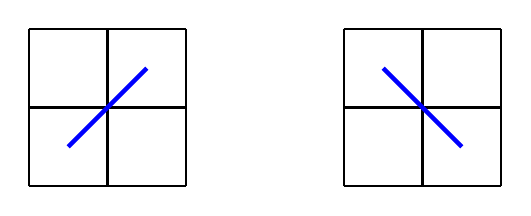
\begin{tikzpicture}[scale=1]
    \draw[step=1.0,black,thick] (0, 0) grid (2, 2);
    \draw[-,ultra thick,blue] (0.5, 0.5) -- (1.5, 1.5);
    \draw[step=1.0,black,thick] (4, 0) grid (6, 2);
    \draw[-,ultra thick,blue] (4.5, 1.5) -- (5.5, 0.5);
  \end{tikzpicture}
  \caption{兩種長鐵路}
  \end{figure}
\end{minipage}
\begin{minipage}{0.5\textwidth}
  \begin{figure}[H]
  \centering
  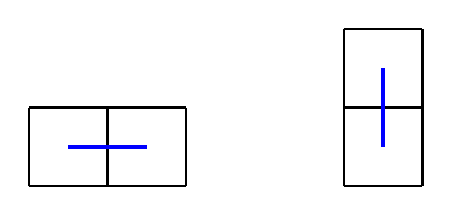
\begin{tikzpicture}[scale=1]
    \draw[step=1.0,black,thick] (0, 0) grid (2, 1);
    \draw[-,ultra thick,blue] (0.5, 0.5) -- (1.5, 0.5);
    \draw[step=1.0,black,thick] (4, 0) grid (5, 2);
    \draw[-,ultra thick,blue] (4.5, 0.5) -- (4.5, 1.5);
  \end{tikzpicture}
  \caption{兩種短鐵路}
  \end{figure}
\end{minipage}

若兩段鐵路共用同一座車站,則稱這兩段鐵路屬於同一條路線,當然\textbf{每座車站都要有一條路線經過}。
另,鋪設多條路線是被允許的,但因成本問題每一條路線\textbf{最多只能有一段長鐵路}。
最後,為了避免外地觀光客坐錯車降低訪問體驗,每條路線都必須是\textbf{環狀}的(確保搭乘順時針或逆時針方向的車都會抵達目的地),且任兩條路線\textbf{不會有任何的重疊或交叉}(意即每座車站皆恰有一條路線經過一次)。

給定古力德市的寬度
\begin{math}L\end{math},請求出有多少種可能的鋪設方式。因為這個數字可能很大,你只要求出鋪設方法數除以
\begin{math}10^9+7\end{math} 的餘數就行了。

以下為 \begin{math}L = 4\end{math} 的範例:在
\begin{math}2 \times 4\end{math} 的地圖中,共有 \begin{math}6\end{math}
種鋪設方式。

\begin{minipage}{0.33\textwidth}
  \begin{figure}[H]
  \centering
  \begin{tikzpicture}[scale=1]
    \def \cycles {
        {0/0/1/0, 1/0/2/0, 2/0/3/0, 3/0/3/1, 3/1/2/1, 2/1/1/1, 1/1/0/1, 0/1/0/0}}
    \draw[step=1.0,black,thick] (0, 0) grid (4, 2);
    \foreach \c in \cycles
    \foreach \xa / \ya / \xb / \yb in \c {
        \def\xc{\directlua{
            tex.sprint(\xa + 0.5)
        }}
        \def\yc{\directlua{
            tex.sprint(\ya + 0.5)
        }}
        \def\xd{\directlua{
            tex.sprint(\xb + 0.5)
        }}
        \def\yd{\directlua{
            tex.sprint(\yb + 0.5)
        }}
        \draw[-,ultra thick,blue] (\xc, \yc) -- (\xd, \yd);
    }
  \end{tikzpicture}
  \end{figure}
\end{minipage}
\begin{minipage}{0.33\textwidth}
  \begin{figure}[H]
  \centering
  \begin{tikzpicture}[scale=1]
    \def \cycles {
        {0/0/1/0, 1/0/1/1, 1/1/0/1, 0/1/0/0},
        {2/0/3/0, 3/0/3/1, 3/1/2/1, 2/1/2/0}}
    \draw[step=1.0,black,thick] (0, 0) grid (4, 2);
    \foreach \c in \cycles
    \foreach \xa / \ya / \xb / \yb in \c {
        \def\xc{\directlua{
            tex.sprint(\xa + 0.5)
        }}
        \def\yc{\directlua{
            tex.sprint(\ya + 0.5)
        }}
        \def\xd{\directlua{
            tex.sprint(\xb + 0.5)
        }}
        \def\yd{\directlua{
            tex.sprint(\yb + 0.5)
        }}
        \draw[-,ultra thick,blue] (\xc, \yc) -- (\xd, \yd);
    }
  \end{tikzpicture}
  \end{figure}
\end{minipage}
\begin{minipage}{0.33\textwidth}
  \begin{figure}[H]
  \centering
  \begin{tikzpicture}[scale=1]
    \def \cycles {
        {0/0/1/0, 1/0/2/0, 2/0/1/1, 1/1/0/1, 0/1/0/0},
        {3/0/3/1, 3/1/2/1, 2/1/3/0}}
    \draw[step=1.0,black,thick] (0, 0) grid (4, 2);
    \foreach \c in \cycles
    \foreach \xa / \ya / \xb / \yb in \c {
        \def\xc{\directlua{
            tex.sprint(\xa + 0.5)
        }}
        \def\yc{\directlua{
            tex.sprint(\ya + 0.5)
        }}
        \def\xd{\directlua{
            tex.sprint(\xb + 0.5)
        }}
        \def\yd{\directlua{
            tex.sprint(\yb + 0.5)
        }}
        \draw[-,ultra thick,blue] (\xc, \yc) -- (\xd, \yd);
    }
  \end{tikzpicture}
  \end{figure}
\end{minipage}

\begin{minipage}{0.33\textwidth}
  \begin{figure}[H]
  \centering
  \begin{tikzpicture}[scale=1]
    \def \cycles {
        {0/0/1/0, 1/0/2/1, 2/1/1/1, 1/1/0/1, 0/1/0/0},
        {2/0/3/0, 3/0/3/1, 3/1/2/0}}
    \draw[step=1.0,black,thick] (0, 0) grid (4, 2);
    \foreach \c in \cycles
    \foreach \xa / \ya / \xb / \yb in \c {
        \def\xc{\directlua{
            tex.sprint(\xa + 0.5)
        }}
        \def\yc{\directlua{
            tex.sprint(\ya + 0.5)
        }}
        \def\xd{\directlua{
            tex.sprint(\xb + 0.5)
        }}
        \def\yd{\directlua{
            tex.sprint(\yb + 0.5)
        }}
        \draw[-,ultra thick,blue] (\xc, \yc) -- (\xd, \yd);
    }
  \end{tikzpicture}
  \end{figure}
\end{minipage}
\begin{minipage}{0.33\textwidth}
  \begin{figure}[H]
  \centering
  \begin{tikzpicture}[scale=1]
    \def \cycles {
        {0/0/1/0, 1/0/0/1, 0/1/0/0},
        {2/0/3/0, 3/0/3/1, 3/1/2/1, 2/1/1/1, 1/1/2/0}}
    \draw[step=1.0,black,thick] (0, 0) grid (4, 2);
    \foreach \c in \cycles
    \foreach \xa / \ya / \xb / \yb in \c {
        \def\xc{\directlua{
            tex.sprint(\xa + 0.5)
        }}
        \def\yc{\directlua{
            tex.sprint(\ya + 0.5)
        }}
        \def\xd{\directlua{
            tex.sprint(\xb + 0.5)
        }}
        \def\yd{\directlua{
            tex.sprint(\yb + 0.5)
        }}
        \draw[-,ultra thick,blue] (\xc, \yc) -- (\xd, \yd);
    }
  \end{tikzpicture}
  \end{figure}
\end{minipage}
\begin{minipage}{0.33\textwidth}
  \begin{figure}[H]
  \centering
  \begin{tikzpicture}[scale=1]
    \def \cycles {
        {0/0/1/1, 1/1/0/1, 0/1/0/0},
        {1/0/2/0, 2/0/3/0, 3/0/3/1}, {3/1/2/1}, {2/1/1/0}}
    \draw[step=1.0,black,thick] (0, 0) grid (4, 2);
    \foreach \c in \cycles
    \foreach \xa / \ya / \xb / \yb in \c {
        \def\xc{\directlua{
            tex.sprint(\xa + 0.5)
        }}
        \def\yc{\directlua{
            tex.sprint(\ya + 0.5)
        }}
        \def\xd{\directlua{
            tex.sprint(\xb + 0.5)
        }}
        \def\yd{\directlua{
            tex.sprint(\yb + 0.5)
        }}
        \draw[-,ultra thick,blue] (\xc, \yc) -- (\xd, \yd);
    }
  \end{tikzpicture}
  \end{figure}
\end{minipage}

\subsection{輸入格式}

\begin{format}
\f{
$L$
}
\end{format}

\begin{itemize}
\tightlist
\item
  \begin{math}L\end{math} 為古力德市的寬度
\end{itemize}

\subsection{輸出格式}

\begin{format}
\f{
$\textrm{ans}$
}
\end{format}

\begin{itemize}
\tightlist
\item
  \begin{math}\textrm{ans}\end{math} 為一整數,代表鐵路鋪設方法數除以
  \begin{math}10^9+7\end{math} 的餘數
\end{itemize}

\subsection{測資限制}

\begin{itemize}
\tightlist
\item
  \begin{math}1 \le L \le 10^{10}\end{math}
\item
  輸入的數皆為整數
\end{itemize}

\subsection{範例測試}

\begin{example}
\exmp{
3
}{%
3
}%
\exmp{
10
}{%
686
}%
\exmp{
327
}{%
265488547
}%
\end{example}

\subsection{評分說明}

本題共有四組子任務,條件限制如下所示。
每一組可有一或多筆測試資料,該組所有測試資料皆需答對才會獲得該組分數。

\begin{longtable}[]{@{}ccl@{}}
\toprule
子任務 & 分數 & 額外輸入限制 \\
\midrule
\endhead
1 & \(10\) & \begin{math}L \le 7\end{math} \\
2 & \(20\) & \begin{math}L \le 10^3\end{math} \\
3 & \(34\) & \begin{math}L \le 10^5\end{math} \\
4 & \(36\) & 無額外限制 \\
\bottomrule
\end{longtable}
